\chapter{Scaling up and distributing}
\label{chap:scalingup}

\begin{abstract}{Abstract}
  Throughout this book, we have been working with examples that consist of
  code to conduct one specific analysis of data sets of modest size.
  But at some point, you may want to scale up. You may want  others
  to be able to  apply your code to their data; and you may want to be able to also
  use your own analyses on larger and more complex datasets. Or you may
  need to run analyses that your own computer cannot deal with.
  This chapter deals with such  steps and points you to some techniques that become increasingly useful
  the larger your projects get.
\end{abstract}

\keywords{databases, cloud computing, containerization, source code, version control}


\begin{objectives}
\item Be able to scale up your analyses
\item Know when to use databases
\item Know when to use cloud computing
\item Know about distributing source code and containers.
\end{objectives}

\begin{feature}
In this chapter, we provide a brief overview of techniques for scaling up computational analyses. In particular, we introduce SQL and noSQL databases, cloud computing platforms, version control systems, and Docker containers.
\end{feature}


%\section{Storing data in SQL and noSQL databases}
\label{sec:databases}

\subsection{When to use a database}
In this book, we have so far stored our data in files. In fact, before
covering the wide range of methods for computational analysis, we
discussed some basics of file handling
(\refchap{filetodata}). Probably, you did not experience any major
trouble here (apart from ocassional struggles with non-standard
encodings, or confusion about the delimiters in a csv file). On the
other hand, the examples we used were still modest in size: usually,
you were dealing with a handful of csv files; except from huge image classification datasets, the maximum you had to
deal with where the 50,000 text files from the IMDB movie review
dataset.

In particular, when loading your data into a dataframe, you copied all
the data from your disk into memory\footnote{In fact, this is
  sometimes a reason to avoid dataframes: for instance, it is possible
  to use a generator that reads data line-by-line from a file and
  yields them to \pkg{scikit-learn}. In this way, only \emph{one} row
  of data is in your memory at the same time (see \refsec{functions}).}
But what if we want to scale up our analyes a bit
\cite[see][]{Trilling2018b}? Maybe we want to build up a larger
datacollection, maybe even share it with multiple team members, search
and filter our data, or collect it over a larger timespan? An
example may illustrate the problems that can arise.

Imagine you do some web scraping (\refchap{scraping}) that goes beyond
a few thousand texts. Maybe you want to visit relevant news sites on a
regular basis (say, once an hour) and retrieve everything that's
new. How do you store your data then? You could append everything to a
huge csv file, but this file would quickly grow so large that you
cannot load it into memory any more. Besides, you may run the risk of
corrupting the file if something goes wrong in one of your attempts to
extend the file. Or you could also write each article to a new, separate file.
That's maybe more failsafe, but you would need to design a good way
to organize the data. In particular, devising a method to search
and find relevant files would be a whole project in itself.

Luckily, you can outsource all these problems to a database that you can
install on your own computer or possibly on a server (in that case, make
sure that it is properly secured!). In the example, the scraper, which
is running once an hour, just sends the scraped data to the database
instead of to a file, and the database will take care of storing it.
Once you want to retrieve a subset of your articles for analysis,
you can send a query to the database and read from it. Both Python and
R offer integration for multiple commonly used databases. It is even
possible to directly get the results of such a database query in
form of a dataframe.

We can distinguish two main categories of databases
that are most relevant to us \citep[see also][]{Gunther2018}:
relational databases (or SQL-databases) and noSQL-databases. Strictly
speaking, SQL (``structured query language'') is a query language for
databases, but it is so widespread that it is used almost synonymously
for relational databases. Even though they have been around for
already 50 years \citep{Codd1970}, relational databases still are very
powerful and very widely used.  They consist of multiple tables that
are linked by shared columns (keys). For instance, you could imagine a
table with the orders placed in a webshop that has a column
|customer-id|, and a different table with addresses, billing
information, and for each |customer-id|. Using filter and join
operations (like in \refchap{datawrangling}, but then on the database directly), one can then easily retrieve
information on where the order has to be shipped. A big advantage of
such a relational database is that, if a customer places 100 orders,
we do not need to store their address 100 times, but only once, which
is not only more efficient in terms of storage, but also prevents
inconsistencies in the data.

In contrast to SQL databases, noSQL databases are not based on tables,
but use concepts such as ``documents'' or key-value pairs, very much
like Python dictionaries or JSON files. These types of databases are
particularly interesting when your data are less well-structured. If
not all of your cases have the same variables, or if the content is not
well-defined (let's say, you don't know exactly in what format the date
of publication on a news site will be written), or if the data structure
may change over time, then it is hard or impossible to come up with a
good table structure for an SQL database. Therefore, in many ``big data''
contexts, noSQL databases are used, as they -- depending on your
configuration -- will happily accept almost any kind of content you dump
in them. This comes, of course, at the expense of giving up advantages
of SQL databases, such as the avoidance of inconsistencies. But often,
you may rather want to store your data first and clean up later, rather
than risking that data collection fails because you enforced a too strict
structure. Also, there are many noSQL databases that are very fast in
searching full text -- something that SQL databases, in general, are
not optimzied for.

Despite all of these differences, both SQL and noSQL databases can play
the same role in the computational analysis of communication. They both
help you to focus on data collection and data analysis without needing
to device an ingenious way to store your data. They both allow for much
more efficient searching and filtering than you could design on your own.
All of this becomes especially interesting when your dataset grows too
large to fit in memory, but also when your data are continuously changed,
for instance because new data are added while scraping.


\subsection{Choosing the right database}
Choosing the right database is not always easy, and has many consequences
for the way you may conduct your analyses. As \citet{Gunther2018} explain,
this is not a purely technical choice, but impacts your social-scientific
workflow. Do you want to enforce a specific structure from the very
start, or do you rather want to collect everything first and clean up
later? What is your tradeoff between avoiding any inconsistency and risking
to throw away too much raw information? 

Acknowledging that there are often many different valid choices, and at
the risk over oversimplifying matters, we will try to give some guidance
in which databases to choose by offering some guiding questions.


\paragraph{How is your data structured?} Ask yourself: Can I organize my data
in a set of relational tables? For instance, think of television
viewing data: There may be a table that gives information on when the
television set was switched on and which channel was watched and by
which user id. A second table can be used to associate personal
characteristics such as age and gender with the user id. And a third
table may be used to map the time stamps to details about a specific
program aired at the time.  If your data looks like this, ask
yourself: Can I determine the columns and the data types for each
column in advance?  If so, then a SQL database such as \pkg{MySQL},
\pkg{PostgreSQL}, or \pkg{MariaDB} is probably what you are looking
for. If, on the other hand, you cannot determine such a structure a
priori, if you believe that the structure of your information will
change over time, or if it is very messy, then you may need a more
flexible, noSQL approach, for instance using \pkg{MongoDB} or
\pkg{ElasticSearch}.

\paragraph{How important is full-text search for you?} SQL databases can handle numeric datatypes as well as text datatypes, but they are usually not optimized for the latter. They handle short strings (such as usernames, addresses, and so on) just fine, but if you are interested in full-text search, they are not the right tool for the job. This is in particular true if you want to be able to do fuzzy searches where, for instance, also documents containing the plural of a word that you searched for as singular are found. Databases of, for instance, news articles, tweets, transcripts of speeches, or other documents are much better accessible in a database such as \pkg{ElasticSearch}.


\paragraph{How flexible does it need to be?} In relational databases, it is relatively hard to change the structure afterwards. In contrast, a noSQL database has no problem whatsoever with adding a new document that contains keys that did not exist before. There is no assumption that all documents contain the same keys. Therefore, if it is hard to tell in advance which ``columns'' or ``keys'' may represent your data best, you should stay clear of SQL databases. In particular, if you think of gradually extending your data and use it on a long timeline for re-use, potentially even by multiple teams, the flexibility of a noSQL database may be a game changer.



\subsection{A brief example using SQLite}

Installing a database server such as \pkg{mysql}, \pkg{mariadb} (an
open-source fork of mysql), \pkg{MongoDB}, or \pkg{Elasticsearch} is
not really difficult (in fact, it may already be come pre-packaged
with your operating system), but the exact configuration and setup may
differ widely depending on your computer and your needs. Most
importantly, especially if you store sensitive data in your database,
you will need to think about authentication, roles, etc. --- all
beyond the scope of this book.

Luckily, there is a compromise between storing your data in files
that you need to manage yourself and setting up a database server,
locally or remotely. The library \pkg{SQlite} offers a self-contained
database engine -- essentially, it allows you to store a whole
database in one file and interact with it using the SQL query language.
Both R and Python offer multiple ways of directly interacting with
sqlite files (\refex{sqlite}). This gives you access to some great
functionality way: after all, you can issue (almost) any SQL command
now, including (and maybe most imporantly) commands for filtering,
joining, and aggregating data. Or you could consider immediately writing
each datapoint you get from an API or a webscraper (\refchap{scraping})
without risking to loose any data if connections time out or scraping
fails halfway.

\pyrex[input=both, output=py, format=table, caption={\pkg{SQLite} offers you database functionality without setting up a database server such as \pkg{mysql}}]{chapter17/sqlite}

Of course, \pkg{SQlite} cannot give you the same performance that a ``real'' mysql (or similar) installation could offer. Therefore, if your project grows bigger, or if you have a lot of read- or
write-operations per second, then you may have to switch at one
point. But as you can see in \refex{sqlite}, Python and R do not
really care about the backend: all you need to do is to change the
connection |conn| such that it points to your new database instead of
the sqlite file.




\section{Storing Data in SQL and noSQL Databases}
\label{sec:databases}

\subsection{When to Use a Database}
In this book, we have so far stored our data in files. In fact, before
covering the wide range of methods for computational analysis, we
discussed some basics of file handling
(Chapter~\ref{chap:filetodata}). Probably, you did not experience any major
trouble here (apart from occasional struggles with non-standard
encodings, or confusion about the delimiters in a csv file). On the
other hand, the examples we used were still modest in size: usually,
you were dealing with a handful of csv files; except for huge image classification datasets, the maximum you had to
deal with were the 50\,000 text files from the IMDB movie review
dataset.

In particular, when loading your data into a dataframe, you copied all
the data from your disk into memory\footnote{In fact, this is
  sometimes a reason to avoid dataframes: for instance, it is possible
  to use a generator that reads data line-by-line from a file and
  yields them to \index{scikit-learn}\emph{scikit-learn}. In this way, only \emph{one} row
  of data is in your memory at the same time (see Section~\ref{sec:functions}).}
But what if we want to scale up our analyses a bit
\cite[see][]{Trilling2018b}? Maybe we want to build up a larger
data collection, maybe even share it with multiple team members, search
and filter our data, or collect it over a larger timespan? An
example may illustrate the problems that can arise.

Imagine you do some web scraping (Chapter~\ref{chap:scraping}) that goes beyond
a few thousand texts. Maybe you want to visit relevant news sites on a
regular basis (say, once an hour) and retrieve everything that's
new. How do you store your data then? You could append everything to a
huge csv file, but this file would quickly grow so large that you
cannot load it into memory any more. Besides, you may run the risk of
corrupting the file if something goes wrong in one of your attempts to
extend the file. Or you could also write each article to a new, separate file.
That's maybe more failsafe, but you would need to design a good way
to organize the data. In particular, devising a method to search
and find relevant files would be a whole project in itself.

Luckily, you can outsource all these problems to a database that you can
install on your own computer or possibly on a server (in that case, make
sure that it is properly secured!). In the example, the scraper, which
is running once an hour, just sends the scraped data to the database
instead of to a file, and the database will take care of storing it.
Once you want to retrieve a subset of your articles for analysis,
you can send a query to the database and read from it. Both Python and
R offer integration for multiple commonly used databases. It is even
possible to directly get the results of such a database query in the
form of a dataframe.

We can distinguish two main categories of databases
that are most relevant to us \citep[see also][]{Gunther2018}:
relational databases (or SQL-databases) and noSQL-databases. Strictly
speaking, SQL (``structured query language'') is a query language for
databases, but it is so widespread that it is used almost synonymously
for relational databases. Even though they have already been around for
 50 years \citep{Codd1970}, relational databases are still  very
powerful and very widely used.  They consist of multiple tables that
are linked by shared columns (keys). For instance, you could imagine a
table with the orders placed in a webshop that has a column
|customer-id|, and a different table with addresses, billing
information, and for each |customer-id|. Using filter and join
operations (like in Chapter~\ref{chap:datawrangling}, but then on the database directly), one can then easily retrieve
information on where the order has to be shipped. A big advantage of
such a relational database is that, if a customer places 100 orders,
we do not need to store their address 100 times, but only once, which
is not only more efficient in terms of storage, but also prevents
inconsistencies in the data.

In contrast to SQL databases, noSQL databases are not based on tables,
but use concepts such as ``documents'' or key-value pairs, very much
like Python dictionaries or JSON files. These types of databases are
particularly interesting when your data are less well-structured. If
not all of your cases have the same variables, or if the content is not
well-defined (let's say, you don't know exactly in what format the date
of publication on a news site will be written), or if the data structure
may change over time, then it is hard or impossible to come up with a
good table structure for an SQL database. Therefore, in many ``big data''
contexts, noSQL databases are used, as they -- depending on your
configuration -- will happily accept almost any kind of content you dump
in them. This comes, of course, at the expense of giving up advantages
of SQL databases, such as the avoidance of inconsistencies. But often,
you may  want to store your data first and clean up later, rather
than risking that data collection fails because you enforced a too strict
structure. Also, there are many noSQL databases that are very fast in
searching full text -- something that SQL databases, in general, are
not optimized for.

Despite all of these differences, both SQL and noSQL databases can play
the same role in the computational analysis of communication. They both
help you to focus on data collection and data analysis without needing
to devise an ingenious way to store your data. They both allow for much
more efficient searching and filtering than you could design on your own.
All of this becomes especially interesting when your dataset grows too
large to fit in memory, but also when your data are continuously changed,
for instance because new data are added while scraping.


\subsection{Choosing the Right Database}
Choosing the right database is not always easy, and has many consequences
for the way you may conduct your analyses. As \citet{Gunther2018} explain,
this is not a purely technical choice, but impacts your social-scientific
workflow. Do you want to enforce a specific structure from the very
start, or do you  want to collect everything first and clean up
later? What is your trade-off between avoiding any inconsistency and risking
 throwing away too much raw information?

Acknowledging that there are often many different valid choices, and at
the risk over oversimplifying matters, we will try to give some guidance
in which databases to choose by offering some guiding questions.


\paragraph[How is your data structured?]{How is your data structured?}
Ask yourself: can I organize my data
in a set of relational tables? For instance, think of television
viewing data: there may be a table that gives information on when the
television set was switched on and which channel was watched and by
which user id. A second table can be used to associate personal
characteristics such as age and gender with the user id. And a third
table may be used to map the time stamps to details about a specific
program aired at the time.  If your data looks like this, ask
yourself: can I determine the columns and the data types for each
column in advance?  If so, then a SQL database such as \index{MySQL}\emph{MySQL},
\index{PostgreSQL}\emph{PostgreSQL}, or \index{MariaDB}\emph{MariaDB} is probably what you are looking
for. If, on the other hand, you cannot determine such a structure \emph{a
priori}, if you believe that the structure of your information will
change over time, or if it is very messy, then you may need a more
flexible, noSQL approach, for instance using \index{MongoDB}\emph{MongoDB} or
\index{ElasticSearch}\emph{ElasticSearch}.

\paragraph[How important is full-text searching for you?]{How important is full-text searching for you?}
SQL databases can handle numeric datatypes as well as text datatypes, but they are usually not optimized for the latter. They handle short strings (such as usernames, addresses, and so on) just fine, but if you are interested in full-text searching, they are not the right tool for the job. This is in particular true if you want to be able to do fuzzy searches where, for instance,  documents containing the plural of a word that you searched for as singular are also found. Databases of, for instance, news articles, tweets, transcripts of speeches, or other documents are much better accessed in a database such as \index{ElasticSearch}\emph{ElasticSearch}.


\paragraph[How flexible does it need to be?]{How flexible does it need to be?}
In relational databases, it is relatively hard to change the structure afterwards. In contrast, a noSQL database has no problem whatsoever with adding a new document that contains keys that did not exist before. There is no assumption that all documents contain the same keys. Therefore, if it is hard to tell in advance which ``columns'' or ``keys'' may represent your data best, you should stay clear of SQL databases. In particular, if you think of gradually extending your data and use it on a long timeline for re-use, potentially even by multiple teams, the flexibility of a noSQL database may be a game changer.



\subsection{A Brief Example Using SQLite}

Installing a database server such as \index{mysql}\emph{mysql}, \index{mariadb}\emph{mariadb} (an
open-source fork of mysql), \index{MongoDB}\emph{MongoDB}, or \index{Elasticsearch}\emph{Elasticsearch} is
not really difficult (in fact, it may already be come pre-packaged
with your operating system), but the exact configuration and setup may
differ widely depending on your computer and your needs. Most
importantly, especially if you store sensitive data in your database,
you will need to think about authentication, roles, etc. --- all
beyond the scope of this book.

Luckily, there is a compromise between storing your data in the files
that you need to manage yourself and setting up a database server,
locally or remotely. The library \index{SQlite}\emph{SQlite} offers a self-contained
database engine -- essentially, it allows you to store a whole
database in one file and interact with it using the SQL query language.
Both R and Python offer multiple ways of directly interacting with
sqlite files (Example~\ref{ex:sqlite}). This gives you access to some great
functionality straight away: after all, you can issue (almost) any SQL command
now, including (and maybe most importantly) commands for filtering,
joining, and aggregating data. Or you could consider immediately writing
each datapoint you get from an API or a webscraper (Chapter~\ref{chap:scraping})
without risking  losing any data if connections time out or scraping
fails halfway.

\pyrex[input=both, output=py, format=table, caption={\index{SQLite}\emph{SQLite} offers you database functionality without setting up a database server such as \index{mysql}\emph{mysql}}]{chapter17/sqlite}

Of course, \index{SQlite}\emph{SQlite} cannot give you the same performance as a ``real'' mysql (or similar) installation could offer. Therefore, if your project grows bigger, or if you have a lot of read-
 or
write-operations per second, then you may have to switch at some
point. But as you can see in Example~\ref{ex:sqlite}, Python and R do not
really care about the back end: all you need to do is to change the
connection |conn| such that it points to your new database instead of
the sqlite file.


%\section{Using cloud computing (CARLOS}
\label{sec:cloudcomputing}


\section{Using Cloud Computing}
\label{sec:cloudcomputing}

Throughout this book, we assumed that all tasks can actually be
performed on your own computer. And often, that is indeed the best
thing to do: you often want to maintain a local copy of your data
anyway, and it may be the safest bet for ethical and legal reasons --
when working with sensitive data, you need to know what you are doing
before transferring them somewhere else.

However, once you scale up your project, problems may arise (see \cite{Trilling2018b}):
\begin{itemize}
\item Multiple people need to work on the same data
\item Your dataset is too large to fit on your disk
\item You do not have enough RAM or processing power
\item Running a process simply takes too long (e.g., training a model
  for several days) or needs to be run in continuous intervals (e.g.,
  scraping news articles once an hour) and you need your computer for
  other things.
\end{itemize}

This is the point where you need to start moving your project to some
remote server instead. Broadly speaking, we can consider three
scenarios:
\begin{enumerate}
\item A cloud service that just lets you run code. Here, you can just
  submit your code and have it run. You do not have full control, you
  cannot set up your own system, but you also do not have to do any
  administration.
\item A dedicated server. You (or your university) could buy a
  dedicated, physical server to run computational social science
  analyses. On the bright side, this gives you full control, but it is
  also not very flexible: after all, you make a larger investment
  once, and if it turns out that you need more (or less) resources,
  then it's too late to change.
\item A virtual machine on a cloud computing platform. For most
  practical purposes, you can do the same as in the previous option,
  with the crucial difference that you rent the resources. If you need
  more, you just rent more; and when you are done, you just stop the
  machine.
\item A set of machines to run complex tasks using parallel computing. With large amounts of information (think about image or video data) and sophisticated modeling (such as deep learning) you may need to distribute the computation among several different computers at the same time.
\end{enumerate}

An example for the first option is Google Colab, which we already used
(Chapter~\ref{chap:fundata}). While it makes it easy to share and run notebooks,
the free tier we used so far does not necessarily solve any of the
scalability issues discussed. However, Google Colab also has a paid Pro
version, in which additional hardware (such as GPUs, TPUs or extra memory)
that you may not have on your own computer can be used. This makes
it an attractive solution for enabling projects (e.g., involving
resource-intensive neural networks) that otherwise would not be possible.

However, this is often not enough. For instance, you may want to run
a database (Section~\ref{sec:databases}) or define a so-called \index{cron}\emph{cron} job,
which runs a specific script (e.g., a web scraper) at defined intervals.
Here, options 2 and 3 come into play -- most realistically for most
beginners, option 3.

There are different providers for setting up VMs in the cloud, the
most well-known probably being Amazon Web Services (AWS) and
Microsoft Azure. Some universities or (national) research infrastructure
providers provide high-performance computing in the cloud as well.
While the specific way to set up a virtual machine of your own on
such an infrastructure varies, the processes are roughly similar:
you select the technical specifications such as the number of CPU
cores and the amount of memory you need, attach some storage, and
select a disk image with an operating system, virtually always some
Linux distribution (Figure~\ref{fig:createvm}).
After a couple of minutes, your machine is ready to use.

\begin{figure}[!tbp]
  \centering
  \begin{minipage}[b]{0.45\textwidth}
    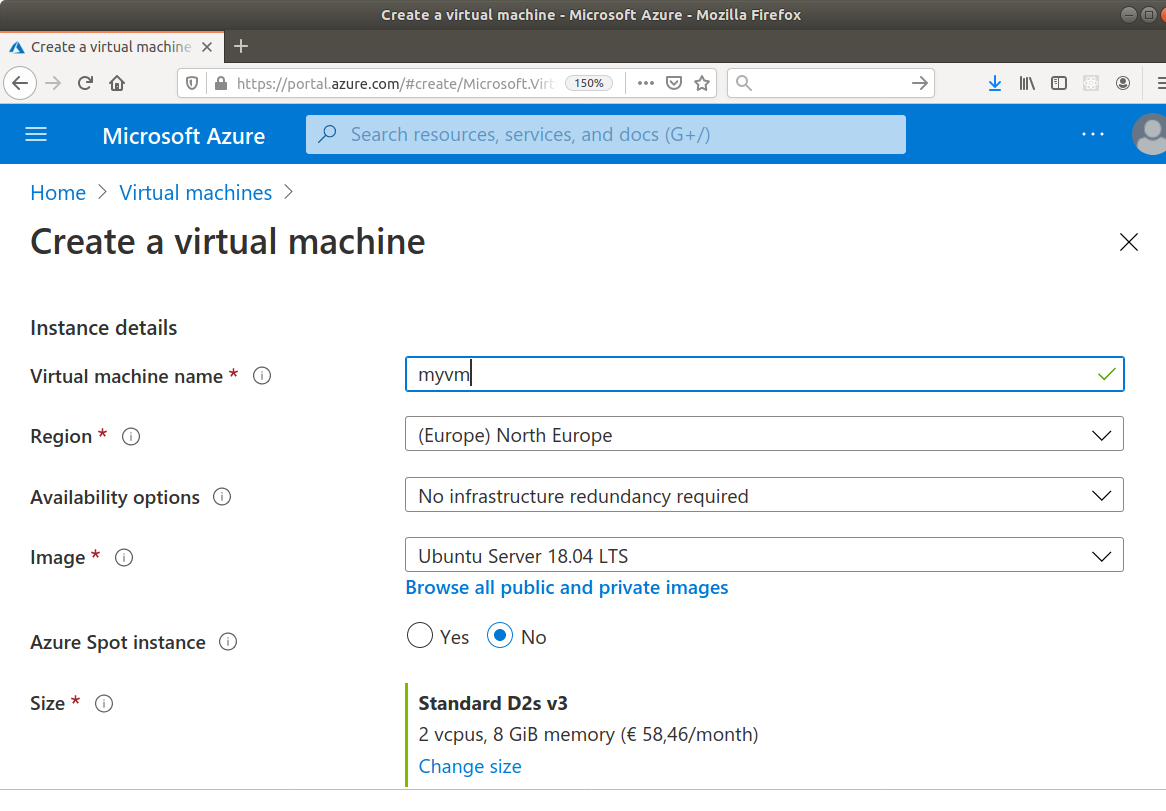
\includegraphics[width=\textwidth]{figures/vmazure.png}
    %\caption{Creating a VM on Microsoft Azure}
  \end{minipage}
  \hfill
  \begin{minipage}[b]{0.45\textwidth}
    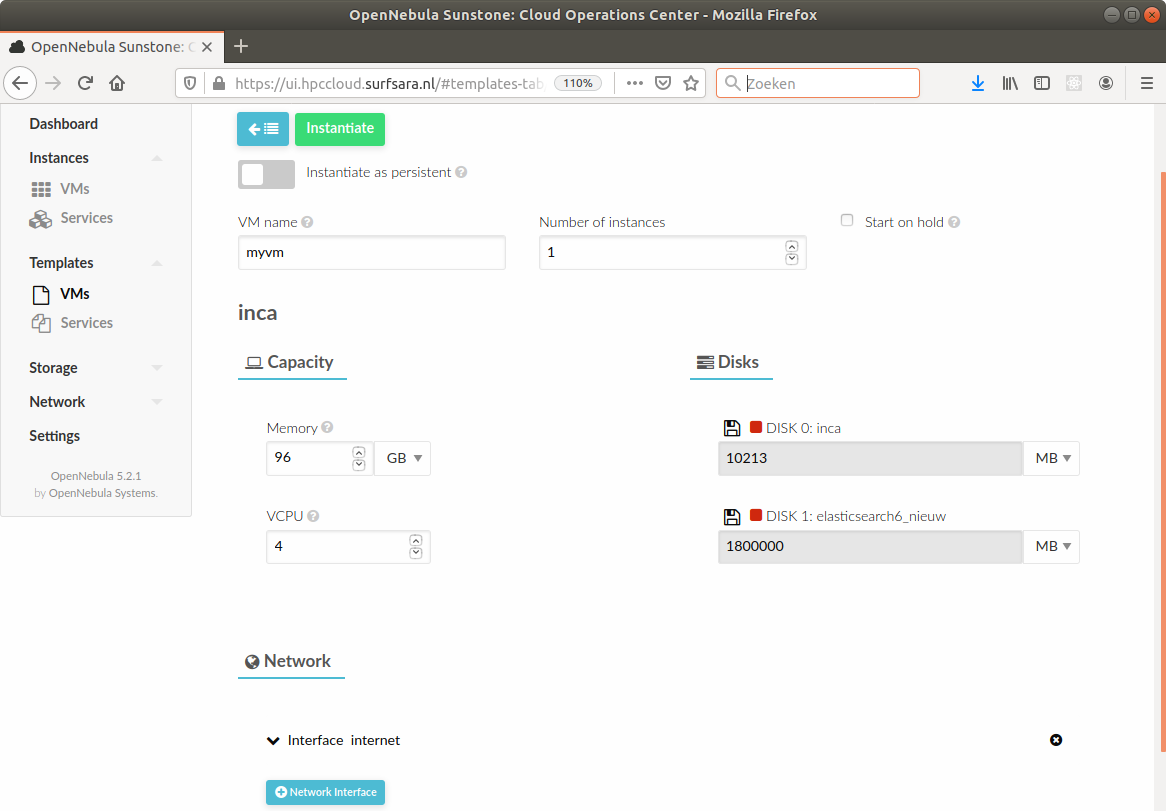
\includegraphics[width=\textwidth]{figures/vmopennebula.png}
    %\caption{}
  \end{minipage}
  \caption{Creating a Virtual Machine on Microsoft Azure (left) and on a university cloud computing platform using OpenNebula (right).\label{fig:createvm}}
\end{figure}

While setting up such a machine is easy, some knowledge is required
for the responsible and safe administration of the machine, in
particular to prevent unauthorized access.

Imagine you have a script |myscript.py| that takes a couple of days to
run. You can then use the tool |scp| to copy it to your new virtual
machine, log on to your virtual machine using |ssh|, and then -- now
on your virtual machine! -- run the script using a tool such as
|nohup| or |screen| that will start your script and will keep running
it (Figure~\ref{fig:ssh}). You can safely logout again, and your
virtual machine in the cloud will keep on doing its work. The only
thing you need to do is collect your results once your script is done,
even if that's a couple of weeks later. Or you may want to add your
script to the crontab (Google it!), which will automatically run
it at set intervals.

\begin{figure}[!tbp]
  \centering
  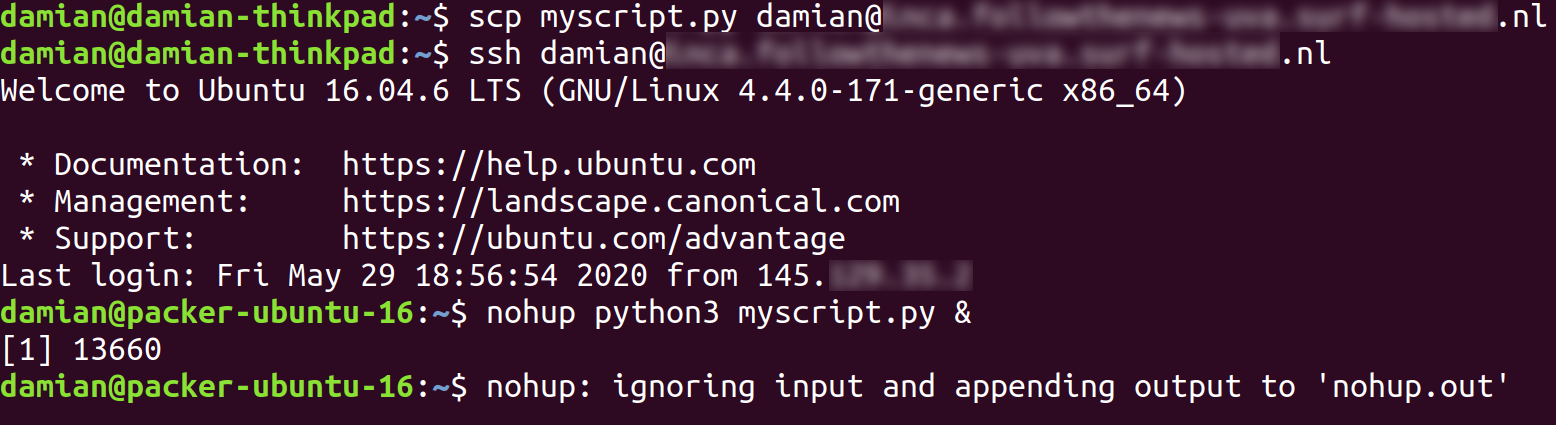
\includegraphics[width=\textwidth]{figures/ssh.png}
  \caption{Running a script on a virtual machine\label{fig:ssh}. Note that the first two commands are issued on the local machine (``damian-thinkpad'') and the next command on the remote machine (``packer-ubuntu-16'').}
\end{figure}

You may want to have some extra luxury, though. Popular things to
set up are databases (Section~\ref{sec:databases}) and \index{JupyterHub}\emph{JupyterHub}, which
allows users such as your colleagues to connect through their
web browser with your server and run their own Jupyter Notebooks
on the machine. Do not forget to properly encrypt all connections,
for instance using \index{letsencrypt}\emph{letsencrypt}.

Finally, option 4 must be selected when the scale of your data and the complexity of the tasks cannot be deployed in a single server or virtual machine. For example, building a classification model by training a complex and deep convolutional neural network with millions of images and update this model constantly may require the use of different computers at the same time. Actually, in modern computers with multiple cores or processors you normally run parallel computing within a single machine. But when working at scale you will probably need to set a infrastructure of different computers such as that of a \textit{grid} or a \textit{cluster}.

Cloud services (e.g., AWS, Microsoft Azure, etc.) or scientific infrastructures (e.g., Supercomputers) offer the possibility of setting up these architectures remotely. For instance, in a computer cluster you can configure a group of virtual computers, where one will act as a \textit{master} and the others as \textit{slaves}. With this logic the master can distribute the storage and analysis of data among the slaves and then resume the results: see for example the \textit{MapReduce} or the \textit{Resilient Distributed Dataset} (RDD) approaches used by the open-source softwares \textit{Apache Hadoop} and \textit{Apache Spark} respectively.

These architectures for parallel processing will significantly increase your computation capacity for big data problems but the initial implementation will consume time and (most of the time) money, which is the reason why you must think in advance if there is a simpler solution (such as single but powerful single machine) before implementing a more complex infrastructure in your analysis.

%\section{Publishing your source}
\label{sec:publishingsource}

Already in \refsec{practices}, we briefly introduced the idea of
version control protocols such as \concept{git}, and the most well-known
online git repostiory \concept{GitHub}.
There are others, such as \concept{Bitbucket}
and the question of which one you use is not really of importance for our
argument here. Already for small projects, it is a good idea to use
version control so that you can always go back to earlier versions,
but as soon as you start working with multiple people on one project,
it becomes indespensable.

In particular, it is possible to work on multiple \emph{branches},
different versions of the code that can later be merged again. In this
way, it is possible to develop new features without interfering with
the main version of the code. There are plenty of git tutorials
available online, and we highly recommended using git from the
beginning of a specific project on -- be it your bachelor, master or doctoral thesis, a paper, or a tool that you want to create.

In the compuational analysis of communication, it becomes more and
more the norm to publish all your source code together with an
article, even though it is important to keep in mind ethical and legal
restrictions (\cite{VanAtteveldt2019}). Using a version control
platform like github from the beginning makes this easy: when
publishing your paper, the only thing you have to do is to set access
of your repository to ``public'' (in case it was private before), add
a |README.md| file (in case you have not done so earlier), and
preferrably, get a persistenant identifier, a |doi| for your
code (see \url{https://guides.github.com/activities/citable-code/}).
And don't forget to add a license to your code, such as MIT, GPL, or
Apache. All of these have specific implications on what others can or
cannot do with your code (e.g., whether it can be used for commercial
purposes or whether derivatives need to be published under the same license as well). Whatever you choose here, it is important \emph{that} you make a choice, as otherwise, it may not be (legally) possible to use
your code at all. 
If your code pertains to a specific paper, then we suggest to organize
your repository as a so-called ``research compendium'', integrating
both your code and your data.
\cite{compendium} provide a template and tools for easily creating one%
\footnote{See url{https://compendium.ccs.amsterdam}}.

In virtually all instances, your code will rely on libraries written
by others, which are available free of charge to you. Therefore,
it only seems fair to ``give back'' and make sure that any code that
you wrote and that can be useful to others, is also available to them.

Just like in the case of a research compendium for a specific paper,
also publishing source code for more generic re-use begins with a
github repository. In fact, both R (with \pkg{devtools}) and Python
(via \pkg{pip}) can install packages directly from github. In order
to make sure that your code can be installed as a package, you
need to follow specific instructions on how to name files, how to
structure your directory, and so on (see \url{https://packaging.python.org/tutorials/packaging-projects/}
and \url{http://r-pkgs.had.co.nz/}).

Regardless of these specific technical instructions, you can make
sure from the outset, though, that your code is easily re-usable.
The checklist below can help making your code publishable from the
outset.

\begin{itemize}
\item Do not hard-code values. Rather than using |"myoutputfile.csv"| or |50| within your script, create constants like |OUTPUTFILE="myoutputfile"| and |NUMBER_OF_TOPICS=50| at the beginning of your script and use these variables instead of the values later on. Even better, let the user provide these arguments as command line arguments or via a configuration file.
\item Use functions. Rather than writing large scripts that are executed from the first line to the last in that order, structure the code in different functions that fulfill one specific task each, and can hence be reused. If you find yourself copy-pasting code, then most likely, you can write a function instead.
\item Document your code. Use docstrings (Python) or comments (R) to make clear what each function does.
\end{itemize}



\section{Publishing Your Source}
\label{sec:publishingsource}

Already in Section~\ref{sec:practices}, we briefly introduced the idea of
version control protocols such as \index{git}\emph{git}, and the most well-known
online git repository \index{GitHub}\emph{GitHub}.
There are others, such as \index{Bitbucket}\emph{Bitbucket}
and the question of which one you use is not really of importance for our
argument here. Already for small projects, it is a good idea to use
version control so that you can always go back to earlier versions,
but as soon as you start working with multiple people on one project,
it becomes indispensable.

In particular, it is possible to work on multiple \emph{branches},
different versions of the code that can later be merged again. In this
way, it is possible to develop new features without interfering with
the main version of the code. There are plenty of git tutorials
available online, and we highly recommended using git from the
beginning of a specific project on -- be it your bachelor, master or doctoral thesis, a paper, or a tool that you want to create.

In the computational analysis of communication, it is becoming more and
more the norm to publish all your source code together with an
article, even though it is important to keep in mind ethical and legal
restrictions (\cite{VanAtteveldt2019}). Using a version control
platform like github from the beginning makes this easy: when
publishing your paper, the only thing you have to do is to set access
of your repository to ``public'' (in case it was private before), add
a |README.md| file (in case you have not done so earlier), and
preferably, get a persistent identifier, a |doi| for your
code (see \url{https://guides.github.com/activities/citable-code/}).
And don't forget to add a license to your code, such as MIT, GPL, or
Apache. All of these have specific implications on what others can or
cannot do with your code (e.g., whether it can be used for commercial
purposes or whether derivatives need to be published under the same license as well). Whatever you choose here, it is important \emph{that} you make a choice, as otherwise, it may not be (legally) possible to use
your code at all.
If your code pertains to a specific paper, then we suggest you organize
your repository as a so-called ``research compendium'', integrating
both your code and your data.
\cite{compendium} provide a template and tools for easily creating one%
\footnote{See url{https://compendium.ccs.amsterdam}}.

In virtually all instances, your code will rely on libraries written
by others, which are available free of charge to you. Therefore,
it only seems fair to ``give back'' and make sure that any code that
you wrote and that can be useful to others, is also available to them.

Just like in the case of a research compendium for a specific paper,
also publishing source code for more generic re-use begins with a
github repository. In fact, both R (with \index{devtools}\emph{devtools}) and Python
(via \index{pip}\emph{pip}) can install packages directly from github. In order
to make sure that your code can be installed as a package, you
need to follow specific instructions on how to name files, how to
structure your directory, and so on (see \url{https://packaging.python.org/tutorials/packaging-projects/}
and \url{http://r-pkgs.had.co.nz/}).

Regardless of these specific technical instructions, you can make
sure from the outset, though, that your code is easily re-usable.
The checklist below can help making your code publishable from the
outset.

\begin{itemize}
\item Do not hard-code values. Rather than using |"myoutputfile.csv"| or |50| within your script, create constants like |OUTPUTFILE="myoutputfile"| and |NUMBER_OF_TOPICS=50| at the beginning of your script and use these variables instead of the values later on. Even better, let the user provide these arguments as command line arguments or via a configuration file.
\item Use functions. Rather than writing large scripts that are executed from the first line to the last in that order, structure the code in different functions that fulfill one specific task each, and can hence be reused. If you find yourself copy-pasting code, then most likely, you can write a function instead.
\item Document your code. Use docstrings (Python) or comments (R) to make clear what each function does.
\end{itemize}


%\section{Distributing your software as container}
\label{sec:container}
When publishing your software, you can think of multiple user
groups. Some may be interested in building on and further developing
your code. Some may not care about your code at all and just want your
software to run. And many others will be somewhere in between.

\emph{Only} publishing your source code (\refsec{publishingsource}) may
be a burden for those who want your code to ``just run'' once your
code becomes more complex and has more dependencies. Imagine a
scenario where your software requires a specific version of
Python or R and/or some very specific (or maybe incompatible) libraries
that you do not want to force the user to install.

And maybe your prospective user does not even know any R or Python.

For such cases, so-called containers are the solution, with as most
prominent platform \pkg{Docker}. You can envision a container as a
minimalistic virtual machine that includes everything to run your
software. To the outside, none of that is visible -- just a network
port to connect to, or a command line to interact with, depending on
your choices.

Software that is containerized using docker is distributed as a
so-called \emph{docker image}. You can build such an image yourself,
but it can also be distributed by pushing it to a so-called registry,
such as the \pkg{Docker Hub}. If you publish your software this
way, the end user has to do nothing else than installing Docker and
running the command |docker run nameofyourimage| - it will be even
downloaded automatically if necessary. There are also GUI versions
of Docker available, which lowers the threshold for some end user
groups even more.

Let's illustrate the typical workflow with a toy example. Imagine
you wrote the following script, |myscript.py|:

\verb|
import numpy as np

from random import randint

a = randint(0,10)

print(f"exp({a}) = {np.exp(a)}")
|

You think that this is an awesome program (after all, it calculates
$e$ to the power of a random integer!), and others should be able
to use it. And you don't want to bother them with setting up Python,
installing numpy, and then running the script. In fact, they do
not even need to \emph{know} that it's a Python program. You
could have written it as well in R, or any other langauge -- for
the user, that will make no difference at all.

What would a docker image that runs this code need to contain? Not
much: First some basic operating system (usually, a tiny Linux distribution),
Python, numpy, and the script itself.

To create such a Docker image, you create a file named |Dockerfile|
in the same directory as your script with the following content:

\texttt{
FROM python:3

ADD myscript.py /

RUN pip install numpy

CMD [ "python", "./myscript.py" ] }


The first line tells Docker to build your new image by starting
from an existing image that already contains an operating system
and Python3. You could also start from scratch here, but this
makes your life much easier. The next line adds your script to the
image, and then we run |pip install numpy| within the image.
The last line just specifies which command with which parameters
needs to be executed when the image is run -- in our case
|python ./myscript.py|.

To create the image, you run |docker build -t dockertest .| (if
you want to name the image ``dockertest''. After that, you can run
it using |docker run dockertest| -- and, if you want to, publish it.

Easy, right?

But when does it make sense to use Docker? Not in our toy example,
of course. While the original code is only a couple of bytes, it now
got bloated to hundreds of megabytes. But there are plenty of
scenarios where this makes a lot of sense.

\begin{itemize}
\item To ``abstract away'' the inner workings of your code. Rather than giving potentially complicated instructions how to run your code, which dependencies to install, etc., you can just provide users with the Docker image, in which everything is already taken care of.
\item To ensure that users get the same results. Though it doesn't form a huge problem on a daily bases for most computational scientists, different versions of different libraries on different systems may occasionally produce slightly different results. The container ensures that the code is run using the same software setup.
\item To avoid interfering with existing installations. Already our toy example had a dependency, \pkg{numpy}, but often, dependecies can be more complex and a program we write may need very specific libraries, or even some other software beyond Python or R libraries. Distributing the source code alone means forcing the user to also install these; and there are many good reasons why people may be reluctant to do so. It may be incompatible with other software on their computer, there may be security concerns, or it just may be too much work. But if it runs inside of the docker container, many of these problems disappear.
\end{itemize}

In short, the Docker image is rarely the \emph{only} way in which you distribute your source code. But already adding a Dockerfile to your github repository so that users can build a Docker container can offer another and maybe better way of running your software to your audience.


\section{Distributing Your Software as Container}
\label{sec:container}
When publishing your software, you can think of multiple user
groups. Some may be interested in building on and further developing
your code. Some may not care about your code at all and just want your
software to run. And many others will be somewhere in between.

\emph{Only} publishing your source code (Section~\ref{sec:publishingsource}) may
be a burden for those who want your code to ``just run'' once your
code becomes more complex and has more dependencies. Imagine a
scenario where your software requires a specific version of
Python or R and/or some very specific (or maybe incompatible) libraries
that you do not want to force the user to install.

And maybe your prospective user does not even know any R or Python.

For such cases, so-called containers are the solution, with as most
prominent platform \index{Docker}\emph{Docker}. You can envision a container as a
minimalistic virtual machine that includes everything to run your
software. To the outside, none of that is visible -- just a network
port to connect to, or a command line to interact with, depending on
your choices.

Software that is containerized using Docker is distributed as a
so-called \emph{Docker image}. You can build such an image yourself,
but it can also be distributed by pushing it to a so-called registry,
such as the \index{Docker Hub}\emph{Docker Hub}. If you publish your software this
way, the end user has to do nothing other than installing Docker and
running the command |docker run nameofyourimage| -- it will even be 
downloaded automatically if necessary. There are also GUI versions
of Docker available, which lowers the threshold for some end user
groups even more.

Let's illustrate the typical workflow with a toy example. Imagine
you wrote the following script, |myscript.py|:

\begin{verbatim}
import numpy as np

from random import randint

a = randint(0,10)

print(f"exp({a}) = {np.exp(a)}")
\end{verbatim}

You think that this is an awesome program (after all, it calculates
$e$ to the power of a random integer!), and others should be able
to use it. And you don't want to bother them with setting up Python,
installing numpy, and then running the script. In fact, they do
not even need to \emph{know} that it's a Python program. You
could have written it as well in R, or any other language -- for
the user, that will make no difference at all.

What would a Docker image that runs this code need to contain? Not
much: first some basic operating system (usually, a tiny Linux distribution),
Python, numpy, and the script itself.

To create such a Docker image, you create a file named |Dockerfile|
in the same directory as your script with the following content:

\texttt{
FROM python:3

ADD myscript.py /

RUN pip install numpy

CMD [ "python", "./myscript.py" ] }


The first line tells Docker to build your new image by starting
from an existing image that already contains an operating system
and Python3. You could also start from scratch here, but this
makes your life much easier. The next line adds your script to the
image, and then we run |pip install numpy| within the image.
The last line just specifies which command with which parameters
needs to be executed when the image is run -- in our case
|python ./myscript.py|.

To create the image, you run |docker build -t dockertest .| (naming
the image ``dockertest''). After that, you can run
it using |docker run dockertest| -- and, if you want to, publish it.

Easy, right?

But when does it make sense to use Docker? Not in our toy example,
of course. While the original code is only a couple of bytes, it now
got bloated to hundreds of megabytes. But there are plenty of
scenarios where this makes a lot of sense.

\begin{itemize}
\item To ``abstract away'' the inner workings of your code. Rather than giving potentially complicated instructions how to run your code, which dependencies to install, etc., you can just provide users with the Docker image, in which everything is already taken care of.
\item To ensure that users get the same results. Though it doesn't form a huge problem on a daily basis for most computational scientists, different versions of different libraries on different systems may occasionally produce slightly different results. The container ensures that the code is run using the same software setup.
\item To avoid interfering with existing installations. Already our toy example had a dependency, \index{numpy}\emph{numpy}, but often, dependencies can be more complex and a program we write may need very specific libraries, or even some other software beyond Python or R libraries. Distributing the source code alone means forcing the user to also install these; and there are many good reasons why people may be reluctant to do so. It may be incompatible with other software on their computer, there may be security concerns, or it just may be too much work. But if it runs inside of the Docker container, many of these problems disappear.
\end{itemize}

In short, the Docker image is rarely the \emph{only} way in which you distribute your source code. But already adding a Dockerfile to your github repository so that users can build a Docker container can offer another and maybe better way of running your software to your audience.

